% !TEX root = deplump.tex
\section{Experiments}
\label{sec:experiments}

The empirical performance of Deplump was evaluated using the most recent Wikipedia content dump as a test corpus.  

\begin{figure*}[t] 
	\begin{center}
		\scalebox{1}{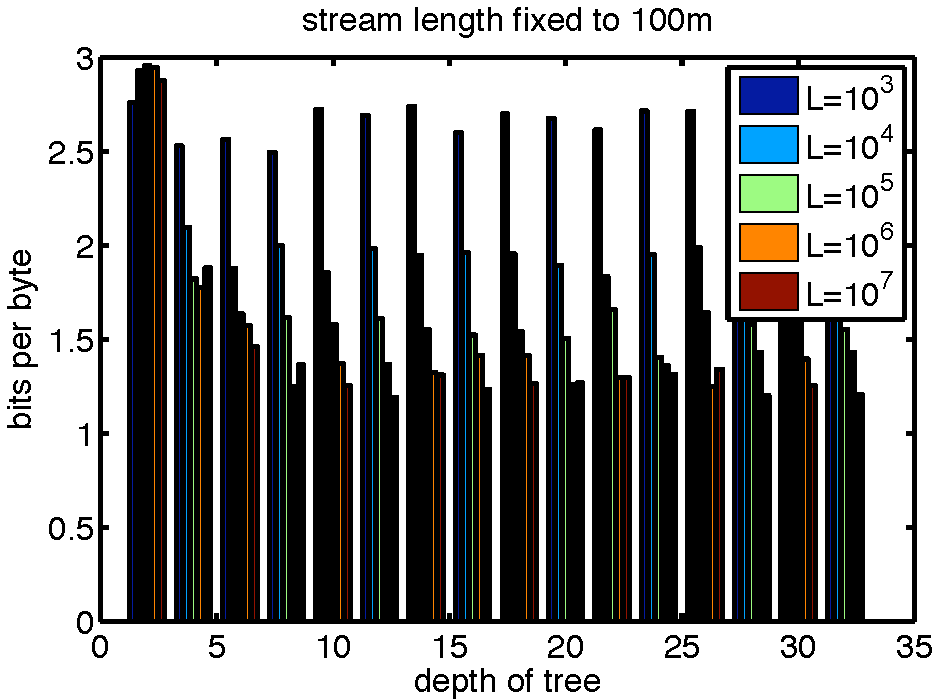
\includegraphics{varying_depths.pdf}} % [clip=true, viewport= 1in 1in 9in 9in]
		\caption{Performance averaged over 10 random sections  100Mb sections of the corpus for varying fixed depths and number of allowable nodes ($L$) }
		\label{fig:varying_depths}
	\end{center} 
\end{figure*} 

\begin{figure*}[t] 
	\begin{center}
		\scalebox{.6}{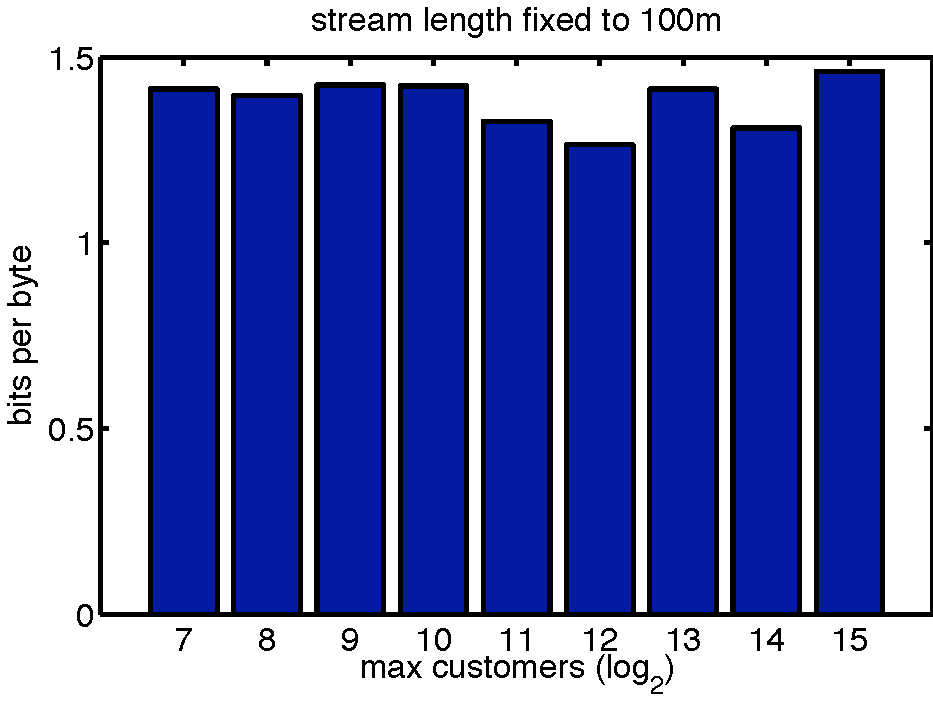
\includegraphics{varying_max_customers.pdf}} % [clip=true, viewport= 1in 1in 9in 9in]
		\caption{Performance for varying max allowable customers $k$.}
		\label{fig: varying_max_customers}
	\end{center} 
\end{figure*} 

\begin{figure*}[t] 
	\begin{center}
		\scalebox{.6}{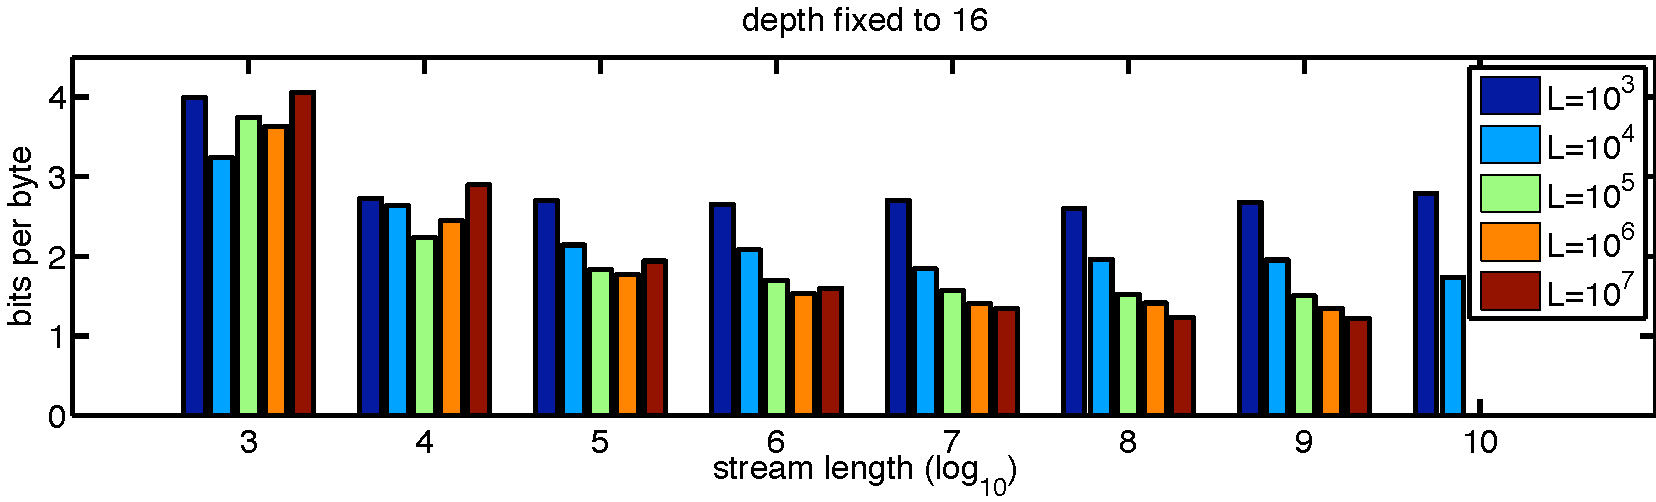
\includegraphics{varying_stream_length.pdf}} % [clip=true, viewport= 1in 1in 9in 9in]
		\caption{Performance for varying stream lengths and number of allowable nodes ($L$).}
		\label{fig:varying_stream_length}
	\end{center} 
\end{figure*} 